\documentclass[sw]{iosart2c}
\usepackage[utf8]{inputenc}
\usepackage[T1]{fontenc}
\usepackage{times}
\usepackage{natbib}
\usepackage{amsmath}
\usepackage{dcolumn}
\usepackage{graphicx}
\usepackage{url}
\usepackage{xspace}
\usepackage{color}
\usepackage{eurosym}
\usepackage{todonotes}
\usepackage[breaklinks]{hyperref}

\def\sectionautorefname{Section}
\def\subsectionautorefname{Section}

\usepackage{multirow}
\usepackage{booktabs}
\usepackage{tabularx}
\usepackage{array}
\usepackage{textcomp}

\newcolumntype{R}{>{\raggedleft\arraybackslash}X}
\newcolumntype{L}{>{\raggedright\arraybackslash}X}
\newcolumntype{C}{>{\centering\arraybackslash}X}

\newcommand{\TODO}[1]{{\color{red}{\textbf{TODO: {#1}}\xspace}}}
\newcommand{\CONSIDER}[1]{{\color{blue}{\textbf{CONSIDER: {#1}}\xspace}}}
\newcolumntype{d}[1]{D{.}{.}{#1}}

\newcommand{\claus}[1]{\todo[inline]{[Claus: #1]}}
%\newcommand{\textrdf}[1]{\texttt{#1}}
\newcommand{\vocab}[1]{\emph{#1}}

\usepackage[scaled]{beramono}
\newcommand\Small{\fontsize{9}{9.2}\selectfont}

\usepackage{listings}
%\lstset{language=Python}
%\lstset{%
% morekeywords={Create,View,As,Construct,With,From}
%}%
\lstset{emph={%  
    Create,View,As,Construct,With,From%
    },emphstyle={\color{blue}\bfseries}%
}%
\lstset{%
    numberbychapter=false,
    numbers=left,
    numberstyle=\tiny,
%    basicstyle=\footnotesize\ttfamily,
    basicstyle=\ttfamily \tiny,
    tabsize=2,
    framexleftmargin=2pt,
    captionpos=b,
    frame=single,
    breaklines=true
}
\lstdefinestyle{rdf}{numberblanklines=true, morekeywords={}}
\lstdefinestyle{sparql}{basicstyle=\ttfamily\scriptsize,numberblanklines=true,
    morekeywords={SELECT,OPTIONAL,FROM,DISTINCT,a,WHERE,FILTER,GROUP,ORDER,LIMIT,BY,IN,AS},
    emph={r,pub,aairObject,verb,person,bday,s,p,o},emphstyle=\textit
}
\lstdefinestyle{turtle}{basicstyle=\ttfamily\tiny ,numberblanklines=true,
    morekeywords={a, @prefix},
    morecomment=[s][\textrm]{<}{>},
    morecomment=[s][\textit]{"}{"},
}

% Default \todo{} to inline mode
\newcommand*{\origtodo}{}
\let\origtodo\todo
\renewcommand*{\todo}{\origtodo[inline]}

\firstpage{1} \lastpage{5} \volume{1} \pubyear{2012}
\begin{document}
\begin{frontmatter} 
\title{Countering language attrition with PanLex and the Web of Data}
\runningtitle{Countering language attrition with PanLex and the Web of Data}

\review{Name Surname, University, Country}{Name Surname, University, Country}{Name Surname, University, Country}

\author[A]{\fnms{Patrick} \snm{Westphal}},
\author[A]{\fnms{Claus} \snm{Stadler}},
\author[B]{\fnms{Jonathan} \snm{Pool}}
\address[A]{University of Leipzig, \{pwestphal, cstadler\}@informatik.uni-leipzig.de}
\address[B]{The Long Now Foundation, San Francisco, pool@panlex.org}

%(%!TEX TS-program = xelatex)
%(%!TEX encoding = UTF-8 Unicode)

\begin{abstract}
At present, there are approximately 7,000 living languages in the world.
However, some forecasters expect the world to lose most of this linguistic diversity.
The mission of the PanLex project is to investigate whether it is feasible to make all languages intertranslatable and thus usable for world-wide communication, and, if so, whether that new situation will interfere with this expected language attrition.
This mission entails, among other prerequisites, making the lexicons of the world's languages intertranslatable. To accomplish that, the project is systematically integrating and making publicly available all known lexical translations.
Semantic Web technologies can enhance the power of PanLex by flexibly representing and reasoning with the content of its database and interlinking it with
%linguistic and
other resources and annotations.
%Using Semantic Web technologies can support achieving this goal, especially due
% to inference capabilities and the interlinking of the PanLex data with other data sources.
Conversely, PanLex, with its unique collection of translation links between more than a billion pairs of lexemes from more than 9,000 language varieties, can improve the coverage of the Linguistic Web of Data.
In this dataset description paper we detail how we transformed the content of the PanLex database to RDF,
established conformance with the lemon and GOLD data models,
interlinked it with Lexvo and DBpedia, and published it as Linked Data and via
SPARQL.
\end{abstract}

\begin{keyword}
Multilingual Linked Open Data, LLOD Cloud, PanLex, Lexical Resource, RDF, RDB2RDF, SPARQL, Sparqlify
\end{keyword}
\end{frontmatter}

\section{Introduction}
\label{sec:intro}
At present, there are about 7,000 living languages in the world\footnote{\url{http://www-01.sil.org/iso639-3/iso-639-3.tab}}.
%\footnote{\url{http://www-01.sil.org/iso639-3/iso-639-3.tab}. As of 25 January 2014, this list contained 6,975 living individual languages.}
%Nonetheless, processes such as urbanization, nation-state consolidation, and globalization appear to be producing language attrition, with, %for example, the extinction or near-extinction in the last 60 years of from 10\% to over 75\% (depending on the world's region) of all living languages\cite{lang_crisis}.
Nonetheless, processes such as urbanization, nation-state consolidation, and globalization appear to be producing language attrition: For example, in the last 60 years and depending on the world's region, from 10\% to over 75\% of all living languages have become extinct or near-extinct~\cite{lang_crisis}.
Theorists of biolinguistic diversity argue that the loss of language diversity, the loss of human biological knowledge, and the loss of species diversity are mutually supportive and thus that language preservation and revitalization are essential to the preservation of biological diversity\cite{nettle}.

The mission of the PanLex project is to investigate the possibility that language attrition would be decreased or halted if utterances in any language were efficiently translatable into all other languages and, as a result, the speakers of all languages could use their languages for world-wide communication. Among the prerequisites of the panlingual translatablity of discourses would be the panlingual translatability of lexicons. In fact, lexical translation is almost the entirety of translation in some contexts (such as personal profiles, bibliographic subject headings, content tagging, product price lists, and web navigation controls). PanLex is designed to support that component by systematically integrating millions of lexical translations, documented in thousands of sources, into a database accessible to the research community, application developers, and the public. The database content can be interpreted as a graph linking millions of lexemes with one another in billions of ``is-a-translation-of'' relations, and permitting intelligent automated inference to trillions more such relations that have not been attested.
%It documents the known lexical translations (translations of lexemes) among all
%languages.

Precisely because the citation forms of lexemes, which is what PanLex directly enables the translation of, are commonly used as labels in collections of data, it is reasonable to speculate that PanLex might facilitate cross-linguistic access to knowledge. The idea of a Semantic Web has led to a stack of technologies standardized by the
\emph{World Wide Web Consortium}\footnote{\url{http://www.w3.org/standards/semanticweb/}}
supporting a machine-readable and machine-interpretable Linked Data
network. This has led to the concept and reality of a \emph{Web of Data}.
%Technologies that support this aim are already available and in use in the so
%called \emph{Web of Data}.
Currently there is a growing community working on leveraging these Semantic Web
technologies for linguistic knowledge and thereby building a Web of Linguistic
Data, also known as the \emph{Linguistic Linked Open Data (LLOD) cloud}.

Our steps to connect PanLex to this Linked Data network are as follows.
In \autoref{sec:triplificate} we introduce the PanLex dataset, present our
PanLex RDF vocabulary, and explain how we transformed the one into the other and established conformance with additional data models.
\autoref{sec:linking} is about how we linked to other datasets of the LLOD cloud,
and \autoref{sec:publishing} is about the publication of the dataset.
Usage scenarios are given in \autoref{sec:usage}.
In \autoref{sec:related} we discuss related work, and finally, in \autoref{sec:conclusion}, we conclude our approach and give some hints about future work.

\section{Triplification of the Raw Data}
\label{sec:triplificate}
In this section, we first provide an analysis of the PanLex dataset.
Subsequently, we introduce our URI and vocabulary design, which closely
resembles PanLex's original conceptual model.
%, which was developed independently from other ontology engineering approaches.
Afterwards, we briefly describe how we classified PanLex's
instance data using additional data models. Finally, we explain the steps
taken to transform the data to RDF.

%As PanLex defines its own  conceptual model 

\subsection{Analysis of the Original Dataset}
\label{sec:analysis}
At the core of the PanLex \emph{project}, there is the PanLex \emph{database}, which is created by editors who consult thousands of lexical sources, such as mono- and multilingual dictionaries, glossaries, standards, and thesauri.
The list of sources that have been and are being consulted is available online\footnote{\url{http://panlex.org/tech/plrefs.shtml}}.
The data based on these sources include single- and multi-word expressions, meanings assigned to them, and related information. Far from being mere copies of the sources, which would not make PanLex data interoperable, the data constitute editors' \emph{interpretations} of various sources' \emph{assertions} that two or more \emph{expressions} share a \emph{meaning}\footnote{\url{http://panlex.org/tech/doc/design/panlex-db-design.pdf}}.
As of January 2014, the database contained about 20 million meanings and 20 million expressions in about 9,200 language varieties based on the consultation of about 1,500 sources by about 20 editors.
The most important entities and relations of PanLex's conceptual model are depicted in \autoref{fig:db-schema} and are explained in more detail below.

\begin{figure}
  \centering
  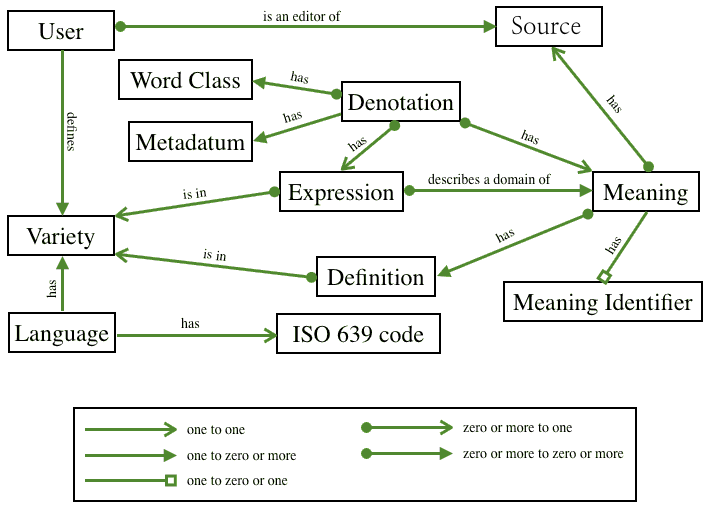
\includegraphics[width=0.4\textwidth]{images/schema-new.png}
  \caption{The PanLex database schema}
  \label{fig:db-schema}
\end{figure}

\todo{The combination of user + source document, which has approved any assertion, is the assertion’s source.}
\begin{itemize}
  \item The starting point of data acquisition is the \emph{source} entity: An editor consults some mono- or multilingual source as mentioned above, interprets it as making assertions about lexical translations, and adds schema-compliant representations of these assertions to the PanLex dataset.
  \item \emph{Expressions} are lexical entities, each defined as a string of characters in some variety of some language. As a first approximation, expressions can be considered lemmas, i.e. dictionary-entry headwords. They differ from traditional headwords, however, in at least two ways. (1) Homographs, such as the verb ``hide'' (conceal) and the noun ``hide'' (animal skin) in English, are treated as a single expression in PanLex. (2) Multiword expressions, such as ``fall in love'', traditionally found in an entry headed by one of their words, such as ``fall'' or ``love'', are treated as independent expressions in PanLex. Expressions are strings of Unicode codepoints subjected to Normalization Form NFC, but this still makes it difficult to search precisely for expressions, so to assist in approximate searching PanLex also adds for each expression a degraded form permitting only lower-case letters and digits.
    \item \emph{Languages} in PanLex are identified using ISO 639-3\footnote{\url{http://www.sil.org/iso639-3/codes.asp}} individual and macrolanguage codes, ISO 639-2\footnote{\url{http://www.loc.gov/standards/iso639-2/}} collective codes, and ISO 639-5\footnote{\url{http://www.loc.gov/standards/iso639-5/}} codes.
    \item \emph {Language varieties} are the fundamental linguistic entities in PanLex. Expressions are in them, not in languages. The language-variety concept is fine-grained and permissive: there can be many varieties of a language, and editors can add varieties as needed. A language variety is identified with some language code, combined with an arbitrary integer differentiating it from other varieties of the same language. For example, six dialects of Ahtna are identified as ``aht-000'' through ``aht-005''. These symbolic 3-letter, 3-digit labels are, themselves, treated as a (controlled) language variety, so editors can clarify their referents by translating them into natural-language expressions and into expressions in other controlled language varieties, such as the IETF standard BCP 47\footnote{\url{http://tools.ietf.org/html/bcp47}}. Such controlled language varieties may be defined as prohibiting synonymy and/or ambiguity.
    \item \emph{Meanings} in PanLex are entities with which expressions are semantically classified. An editor documents that two or more expressions are asserted to be translations or synonyms of one another by assigning a shared meaning to them. For example, depending on an editor's judgment, a source's translation of the German lexeme ``klingen'' into a sequence of alternative English lexemes ``ring, sound, seem'' can be documented by either (1) the assignment of all four expressions to the same meaning or (2) the assignment of two or three meanings to ``klingen'' and of one of those meanings to each of the English expressions. For practicality, PanLex treats expressions and meanings asymmetrically. Newly added translations automatically re-use existing matching expressions, but they don't re-use existing meanings, because there is no straightforward test of equivalence for meanings. PanLex generates new meanings as needed, and meanings are source-specific, leaving it for subsequent research to investigate which meanings should be considered equivalent and thus consolidated. Meanings can further have properties of three types. (1) \emph{Definitions} are descriptions of a meaning, consisting of arbitrary text strings annotated as being in particular language varieties. (2) \emph{Domains} are expressions (e.g., ``medicine'') that classify a meaning, but do not express it. (3) \emph{Meaning identifiers} are strings acting as references to identifiers used in a source.
    \item \emph{Denotations} are assignments of meanings to expressions. Each denotation, in addition to its meaning-expression pair, may be assigned one or more \emph{word classes} (a closed set based on OLIF, the Open Lexicon Interchange Format) and/or \emph{metadata} (arbitrary strings paired as keys and values).
    %For example, \emph{fall} can be a verb or a noun for autumn.
    %Homonyms are those expressions that are connected to multiple meanings.
  \item \emph{Users} are the entities that may act as editors by defining sources and then defining data attributed to those sources, as well as defining language varieties.
  \item Sources in PanLex are defined with about two dozen properties, among them being \emph{licenses}. As of January 2014 eleven different license categories were recognized. They were \emph{public domain}, \emph{Creative Commons (CC)}, \emph{request} (meaning that one has to ask the author of the resource), \emph{GNU General Public License (GPL)}, \emph{GNU Lesser General Public License (LGPL)}, \emph{GNU Free Documentation License (FDL)}, \emph{MIT License}, \emph{copyright} (meaning that there is a copyright claim without a more liberal license also being offered), \emph{PanLex Use Permission} (where an author or publisher has given a source to PanLex for its use), \emph{other}, and \emph{unknown}.
    The distribution of licenses among sources that had been or were being consulted in January 2014 is shown in \autoref{tbl:plx-license-counts}.
\end{itemize}

\begin{table}
\centering
\begin{scriptsize}
\begin{tabular}{lrclrclr}
License          & Count &&
License          & Count &&
License          & Count \\
\cline{1-2} \cline{4-5} \cline{7-8}
\emph{copyright} &  1343  && \emph{LGPL}      &     9 && \emph{PD}           & 149 \\
\emph{CC}          &   387   && \emph{MIT}         &    32 && \emph{other}       &   106 \\
\emph{FDL}        &    24    && \emph{PanLex}    &    7 && \emph{unknown}  &  1958 \\
\emph{GPL}        &   172   && \emph{request}    &     5 \\
\end{tabular}
\end{scriptsize}
\caption{Number of sources using a certain license}
\label{tbl:plx-license-counts}
\end{table}

An overview of the number of instances per entity as of January 2014 is given in~\autoref{fig:plx-entity-counts}.
\begin{table}
  \centering\begin{scriptsize}
  \begin{tabular}{lrclr}
    Entity             & Instances  \\
    \cline{1-2}
    Denotations        & 54,278,860 \\  % SELECT COUNT(dn) FROM dn;
    Languages          &      7,843 \\ % SELECT COUNT(lc) FROM lc; -- all language codes (ISO 639-3, ISO 639-2, ISO 639-5) known in the PanLex db
    Language Varieties identified           &      9,310 \\  % SELECT COUNT(lv) FROM lv;
    Language Varieties with data           &      9,239 \\  % 
    Meanings           & 20,773,371 \\  % SELECT COUNT(mn) FROM mn;
    Sources being consulted         &      4,190 \\  % 
    Sources already consulted         &      1,453 \\  % 
    Expressions        & 19,790,453 \\ % SELECT COUNT(ex) FROM ex;
    Definitions        &  2,747,892 \\ % SELECT COUNT(df) FROM df;
    Users              &          23 \\ % SELECT COUNT(us) FROM us;
  \end{tabular}
  \end{scriptsize}
  \caption{Number of instances of main entities in the PanLex database}
  \label{fig:plx-entity-counts}
\end{table}

\subsection{The PanLex vocabulary}
\label{sec:vocabulary}
The entities and relations of the schema described in the previous section serve as the base for the development of the PanLex RDF vocabulary.
In general, all PanLex RDF resources reside in the namespace \texttt{\small <http://ld.panlex.org/plx/>}, abbreviated with \texttt{\small plx}.
An example of the resulting ontology is depicted in \autoref{fig:vocabulary} and summarized as follows.
Unless otherwise noted, the URIs of instances of PanLex classes follow the pattern \emph{plx:\{className\}/\{id\}}, where \{className\} is spelled in lower camel case and the \{id\} is the primary key of the corresponding database table.

\begin{itemize}
  \item Expressions are modeled as instances of the class \texttt{\small plx:Expression}.
    Their original and degraded textual representations become the values of the properties \texttt{\small rdfs:label} and \texttt{\small plx:degradedText}, respectively.
    Their corresponding language variety is stated using \texttt{\small plx:languageVariety}.
  \item For language and language varieties the classes \texttt{\small plx:Language} and \texttt{\small plx:LanguageVariety} are introduced.
    \emph{ISO 639-1} and \emph{ISO 639-3 codes} become instances of the classes \texttt{\small plx:Iso639-1Code} and \texttt{\small plx:Iso639-3Code}.
  \item The RDF analog of the PanLex \emph{meaning} is the \texttt{\small plx:Meaning}.
    Entities of this class may have an identifier assigned with the \texttt{\small plx:identifier} property pointing to an \texttt{\small xsd:string} literal.
    Meanings may also have \emph{definitions}, entities of the \texttt{\small plx:Definition} class, giving a textual representation (\texttt{\small rdfs:label}) in a certain language variety (\texttt{\small plx:languageVariety}).
  \item Following the semantics of the PanLex database, meanings and expressions are linked via \emph{denotations}.
    These are entities of the \texttt{\small plx:Denotation} class pointing to meanings and expressions via the properties \texttt{\small plx:denotationMeaning} and \\ \texttt{\small plx:denotationExpression}.
    Denotations may also have a word class assigned to them.
    This can be achieved with the denotation's \texttt{\small plx:wordClass} property pointing to a \texttt{\small plx:WordClass} entity.
  \item All sources share the \texttt{\small plx:Approver} class.
    The characteristics of a source are described using mainly triples with literal objects.
    These are for example \texttt{\small dc:title} to assign the title of a source, \texttt{\small dc:creator} to give an \texttt{\small xsd:string} containing the author's name. At present, we support the different license categories recognized in the database by creating resources of the \texttt{\small plx:License} class.
\end{itemize}

\begin{table}
  \begin{tiny}
  \begin{tabular}{p{52px}p{140px}}
    Class                 & Properties \\
    \toprule
    \texttt{plx:Approver} & \mbox{\texttt{plx:registrationDate}, \texttt{rdfs:label}, \texttt{dc:title},}
                            \mbox{\texttt{dc:creator}, \texttt{plx:license}, \texttt{dc:date}, \texttt{plx:quality},}
                            \mbox{\texttt{foaf:homepage}, \texttt{dc:publisher}, \texttt{dbpedia-owl:isbn}} \\
    \midrule
    \texttt{plx:Language} & \texttt{plx:iso639-3Code}, \texttt{plx:iso639-1Code} \\
    \midrule
    \texttt{plx:LanguageVariety}
                          & \texttt{plx:languageVarietyOf}, \texttt{rdfs:label} \\
    \midrule
    \texttt{plx:Iso639-1Code} & \\
    \midrule
    \texttt{plx:Iso639-3Code} & \\
    \midrule
    \texttt{plx:Expression}
                          & \mbox{\texttt{plx:languageVariety}, \texttt{plx:degradedText},} \texttt{rdfs:label} \\
    \midrule
    \texttt{plx:Meaning}
                          & \mbox{\texttt{plx:approver}, \texttt{plx:identifier},} \texttt{plx:meaningDefinition} \\
    \midrule
    \texttt{plx:Definition}
                          & \texttt{plx:languageVariety}, \texttt{rdfs:label} \\
    \midrule
    \texttt{plx:Denotation}
                          & \texttt{plx:denotationMeaning}, \texttt{plx:denotationExpression}, \texttt{plx:wordClass} \\
    \midrule
    \texttt{plx:WordClass}  
                          & \texttt{rdfs:label} \\
    \midrule
    \texttt{plx:License}  & \texttt{rdfs:label} \\
    \bottomrule
  \end{tabular}
  \end{tiny}
  \caption{Classes and properties used in the PanLex RDF vocabulary. Note that all \texttt{rdf:type} properties are omitted for brevity.}
  \label{tbl:vocabulary}
\end{table}

\begin{figure}
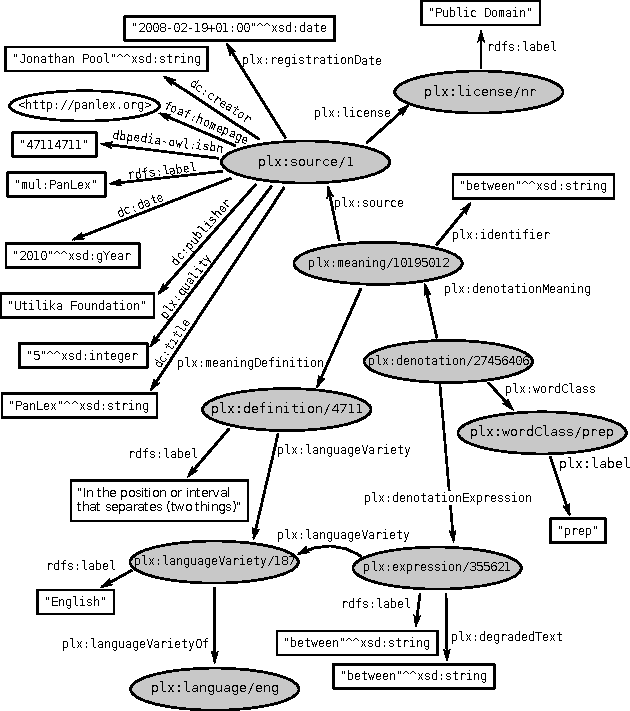
\includegraphics[width=0.46\textwidth]{images/pdf/ontology.pdf}
\caption{Overview of the PanLex RDF vocabulary}
\label{fig:vocabulary}
\end{figure}

\begin{table}
  \centering\begin{scriptsize}
  \begin{tabular}{p{48px}p{62px}p{70px}}
    Panlex                  & lemon                       & GOLD \\
    \midrule
    \texttt{plx:Denotation} & --                          & \texttt{gold:LinguisticSign} \\
    \texttt{plx:Meaning}    & \texttt{lemon:LexicalSense} & \texttt{gold:SemanticUnit} \\
    \texttt{plx:Expression} & \texttt{lemon:LexicalEntry} & \texttt{gold:FormUnit} \\
  \end{tabular}
  \end{scriptsize}
  \caption{Classes considered to be similar across the re-used vocabulary}
  \label{tbl:sameclasses}
\end{table}

\subsection{Vocabulary Reuse}
\label{sec:vocabulary-reuse}
The PanLex vocabulary is based on PanLex's conceptual schema and
enables all of PanLex's data to be directly exposed as RDF.
%Apart from modeling a PanLex RDF vocabulary
Additionally, we also re-use existing vocuabularies, namely
the \emph{Lexicon Model for Ontologies} (lemon)~\cite{lemon2011} as well as the \emph{General Ontology for Linguistic Description} (GOLD)~\cite{farr2003}.
Since these models differ from the PanLex one to some extent, we follow an
incremental approach of aligning the PanLex data with them.
%accordingly. 
% one differ to some
%extend, not the whole schemas were implemented.
\autoref{tbl:sameclasses} shows PanLex classes with their current counterparts
in lemon and GOLD respectively.
The parts implemented in our RDF conversion are displayed in \autoref{fig:goldlemonimplemented}.
\begin{figure}
  \centering
  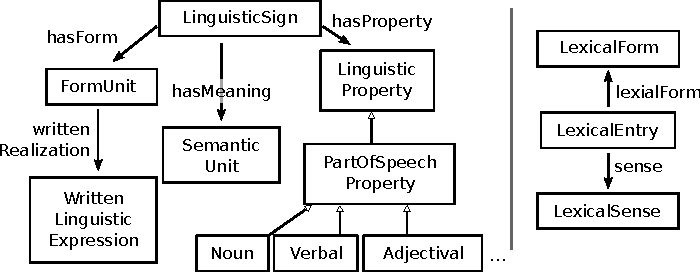
\includegraphics[width=\linewidth]{images/pdf/gold_lemon_implemented.pdf}
  \caption{Parts of the GOLD (left) and lemon model (right) re-used in PanLex (URI prefixes are omitted for brevity)}
  \label{fig:goldlemonimplemented}
\end{figure}

\subsection{Transformation workflow}
\label{sec:conversion}
Since new sources are added to the PanLex database on almost a daily basis and because of its current size (\textasciitilde18 GB), the recurrent conversion of the database to capture changes in it is impractical.
%Using conventional hardware, a full conversion takes infeasibly long.
%This makes the testing and debugging of the modeled vocabularies and data very
% time-consuming.
As the PanLex data already reside in a relational database, the use of a virtual RDB2RDF\footnote{\url{http://www.w3.org/2001/sw/wiki/RDB2RDF}} mapping solution is a natural choice.
The \emph{Sparqlify system}\footnote{\url{https://github.com/AKSW/Sparqlify}} offers, besides an efficient query rewriting engine, also a very easy-to-use mapping language, called \emph{Sparqlification Mapping Language} (SML).
Essentially, these mappings consist of three clauses:
The \emph{From} clause specifies the logical SQL table (i.e. table, view, or
query) to be used in the SML view.
The \emph{With} clause binds a set of SPARQL variables to expressions that
yield RDF terms from relational columns.
Finally, the \emph{Construct} clause holds a set of triple patterns.
%clause making use of the defined SPARQL variable definitions.
\autoref{fig:ex:sparqlify-ml} shows an example of an SML view for the
languages in PanLex: From each row of the table \emph{i1} three resources are
created based on the \emph{iso3} column and 
bound to the variable names \emph{?lang}, \emph{?iso3} and \emph{?lexvo3}.
Resources for \emph{?lang} become typed as a \emph{Language} in the PanLex and the \emph{schema.org} namespace.
This view-based approach also demonstrates that changing the vocabulary or
adding support for new ones does not require an extract transform load (ETL) process,
and can therefore be done with little effort.

\begin{figure}
\centering
\begin{lstlisting}
Create View i1 As Construct {
    ?lang a plx:Language, <http://schema.org/Language> ;
          plx:iso639-3Code ?iso3 .
    ?iso3 a plx:Iso639-3Code ;
          owl:sameAs ?lexvo3 .  }
  With
      ?lang = uri(plx:language, '/', ?iso3)
      ?iso3 = uri(plx:iso639-3, '/', ?iso3)
      ?lexvo3 = uri('http://lexvo.org/id/iso639-3/', ?iso3)
  From [[SELECT iso3 FROM i1]]
\end{lstlisting}
\caption{An excerpt of an SML view definition for PanLex's languages. This
example also demonstrates how ``is-a'' relations to schema.org and links to Lexvo are established.}
\label{fig:ex:sparqlify-ml}
\end{figure}

\section{Linking}
\label{sec:linking}
The SML view in the previous section (\autoref{fig:ex:sparqlify-ml}) already established the interlinking of the PanLex languages with Lexvo.
In this section we outline the interlinking with DBpedia.
For DBpedia, we were interested in creating \emph{valid} and thus \emph{dereferenceable} links.
Therefore, we iterated the \emph{titles} datasets\footnote{\url{http://wiki.dbpedia.org/Downloads38}}, which map (non-localized) DBpedia URIs to their page titles in the respective language.
For each language version we normalized the labels by applying Unicode NFKD\footnote{\url{http://unicode.org/reports/tr15/}} normalization and removal of punctuation characters.
Each DBpedia resource was then mapped to the PanLex expression that was equal to the resource's normalized label in the respective language.
\autoref{fig:plx-dbp-link-counts} summarizes the number of links obtained.

In total, about 2.5 million links were obtained for approx. 20 million expressions.
This relatively low coverage can be attributed to frequently appearing multi-word expressions that do not match the DBpedia titles well, and the fact that in this work we yet only considered DBpedia datasets for mainstream languages, whereas PanLex focuses on low-density ones.

\begin{table}
  \centering\begin{scriptsize}

  \begin{tabular}{lrclr}
    Language   &   Links   && Language  & Links     \\
    \cline{1-2}\cline{4-5}
    English    & 1,415,241 && Catalan   &    27,779 \\
    German     &   224,146 && Korean    &    24,912 \\
    French     &   187,364 && Turkish   &    22,258 \\
    Italian    &   147,485 && Bulgarian &    19,431 \\
    Spanish    &   117,056 && Hungarian &    18,203 \\
    Portuguese &   112,266 && Slovene   &    11,981 \\
    Polish     &   110,974 && Greek     &     1,112 \\
    \cline{4-5}
    Russian    &    68,040 \\
    Czech      &    28,767 && Total     & 2,537,015 \\
  \end{tabular}
  \end{scriptsize}
  \caption{Number of DBpedia links per language}
  \label{fig:plx-dbp-link-counts}
\end{table}

\section{Publishing}
\label{sec:publishing}
With our RDF conversion work, we complement existing
APIs\footnote{\url{http://panlex.org/try/}} with Linked Data, powered by
Pubby\footnote{\tiny{\url{http://wifo5-03.informatik.uni-mannheim.de/pubby/}}},
and two SPARQL
endpoints\footnote{\url{http://ld.panlex.org/vsparql}}
\footnote{\url{http://ld.panlex.org/sparql}}, powered by Sparqlify and Virtuoso,
respectively.
% and \url{http://ld.panlex.org/snorql}}.
An overview is shown in ~\autoref{fig:panlex-architecture}.
The SPARQL browser
\emph{SNORQL}\footnote{\url{https://github.com/kurtjx/SNORQL}} can be accessed
by replacing \emph{sparql} with \emph{snorql} in the respective links. Our SML
views and the interlinking code are hosted on GitHub\footnote{\url{https://github.com/AKSW/PanLex-2-RDF}}.
The created linksets are hosted in the PanLex database and are published together with the other data using the Sparqlify RDB2RDF tool.
Finally, we offer downloads tagged with timestamps of their creation\footnote{\url{http://ld.panlex.org/downloads/releases/}}.
\begin{figure}
\centering
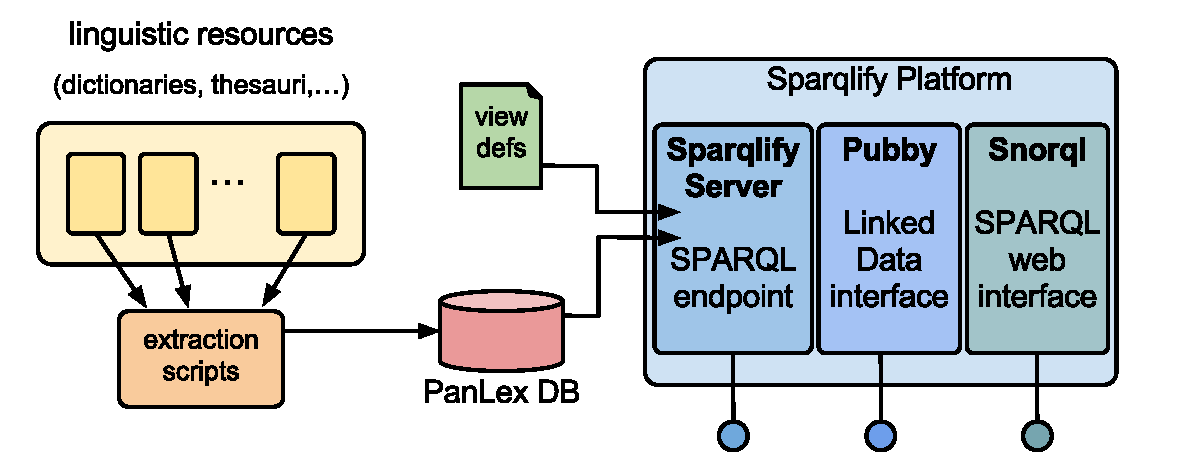
\includegraphics[width=0.5\textwidth]{images/pdf/sparqlify_setup02.pdf}
\caption{PanLex architecture}
\label{fig:panlex-architecture}
\end{figure}

\section{Dataset Benefits and Usage Scenarios}
\label{sec:usage}
There are general benefits of using Semantic Web technologies, such as the
potential for simplified data integration due to RDF and vocabulary reuse, the
possibility of enriching data based on interlinking, drawing advantage from
reasoning and the exploration of the data through the use of generic Semantic
Web tools.
Moreover, some applications, like the TeraDict translation lookup
service\footnote{\url{http://panlex.org/teradict/?lg=eng}}, can now be realized
using SPARQL queries and so easily integrated in other applications.
Due to space considerations, we refer the reader to the PanLex Linked Data
landing page\footnote{\url{http://ld.panlex.org}}, where a
collection of SPARQL queries is maintained.
Also, since PanLex covers a niche of providing linguistic data for
non-mainstream languages, investigation of its fitness for use in cross
language information retrieval, as well as annotation projects, like DBpedia
Spotlight\footnote{\url{http://spotlight.dbpedia.org}}, seems worthwhile.

%exploiting data of projects like Wordnet, e.g. via the LemonWordNet
% dataset\footnote{\url{http://datahub.io/de/dataset/lemonwordnet}} can help
 % finding errors or derive new data and improve translations.
%Another source that could be combined with the PanLex data is the Wortschatz project\footnote{\url{http://wortschatz.uni-leipzig.de/}}.
%Using Wortschatz's co-occurrences statistics of words in different languages one could also improve the recall of word-by-word translations.

%(see \autoref{lst:terradict} for an example).

%that currently only support mainstream languages.
%Apart from this users can easily explore the PanLex data using the
%Linked Data and SPARQL services.
%This also increases the chance of development of new interesting mashups.
% vision web of data
%% \begin{figure}
%% \centering
%% \begin{lstlisting}
%% SELECT ?expr_lbl WHERE {
%%     ?expr_lang rdfs:label "language" .
%%     ?denotation_lang plx:denotationExpression ?expr_lang .
%%     ?denotation_lang plx:denotationMeaning ?meaning .
%%     ?denotation_other plx:denotationMeaning ?meaning .
%%     ?denotation_other plx:denotationExpression ?expr_other .
%%     ?expr_other rdfs:label ?expr_lbl .
%%     FILTER(?expr_lang != ?expr_other)
%% }
%% \end{lstlisting}
%% \caption{SPARQL query to retrieve all known lexical translations of the given English word \emph{`language'}}
%% \label{lst:terradict}
%% \end{figure}

\section{Related Work}
\label{sec:related}
PanLex is a project whose editors integrate information discovered from many lexical resources.
The extraction of information from linguistic sources, and techniques for automatically inferring translations,
are relevant work discussed in \cite{panlex_probtrans}.
%A similar approach of linking expressions to meanings is followed by the
% \emph{Global Wordnet Association}.
An important related initiative is the Global Wordnet Association\footnote{\url{http://www.globalwordnet.org/}\vspace{0.7em}},
which offers a platform for sharing wordnets and, among other goals, uniformly representing wordnets
of different languages and establishing a universal index of meaning.
Wordnets are usually focused on the
definition of \emph{synsets} and relations between them in a single language; GWA is helping to transform these single-language synonym silos into a virtual multilingual translation resource. PanLex is approximating that, in a different way, by integrating data from numerous wordnets along with translingual sources into a single graph.
%As already mentioned in PanLex there can be several meaning entities
% representing the same unique sense.
In the Semantic Web context, several standard or quasi-standard vocabularies and ontologies have been developed with the rise of the \emph{Linguistic Linked Open Data} movement.
Examples include the
\emph{Ontologies of Linguistic Annotation} (OLiA)~\cite{olia2010} for modeling
lexicon and machine-readable dictionaries, \emph{POWLA} for modeling linguistic corpora\cite{powla2012} and the \emph{Natural Language Processing Interchange Format} (NIF)\footnote{\url{http://nlp2rdf.org/nif-1-0}}.

\section{Conclusions and Future Work}
\label{sec:conclusion}
In this dataset description we detailed the PanLex database and its conversion to RDF.
Based on our URI and vocabulary design, we created appropriate view definitions
for the \emph{Sparqlify} system, which carries out the actual RDF
transformation.
Furthermore, we interlinked the languages in PanLex with Lexvo, and created about 2.5 million links to DBpedia for expressions in 16 languages.
With the integration of lemon and GOLD we also support data access via external linguistic ontologies.

We intend to address some limitations in the future. Attribution is currently limited to sources, obscuring the possible roles of multiple editors in iteratively interpreting sources and the subsidiary sources of data in sources that are themselves aggregations. Metadata attached to PanLex denotations are currently limited to arbitrary pairs of strings, but this sacrifices discovery possibilities when the metadata (as they often do) describe facts that can be expressed with PanLex expressions (e.g., that the expression is archaic). New collaborations between PanLex and related standards and technologies (e.g., language identification, language geolocation, lemmatization, transliteration, localization, etc.) are promising arenas for development. For example, the relations among PanLex's information sources, if treated as distinct datasets, could be modeled with the VoID vocabulary\footnote{\url{http://rdfs.org/ns/void}}.

\bibliographystyle{abbrv}
\bibliography{bibliography,../../bib/aksw}
\end{document}
